
\section{Simulation of the MPPT algorithm} \label{MPPTSimulation}

The results obtained in simulation for the previously explained P\&O algorithm will be shown in this section. First, the results corresponding to the PV panel model will be evaluated without connecting it to the DC-DC converter. Once the model for the PV panel is validated, the results obtained for the complete system will be analyzed in order to show the performance of the MPPT algorithm under different environmental conditions and resistive loads \todo{Confirm with the supervisors if resistive load or voltage source}.  

\subsection{Model of the PV panel}

\begin{figure}[H]
	\begin{center}
		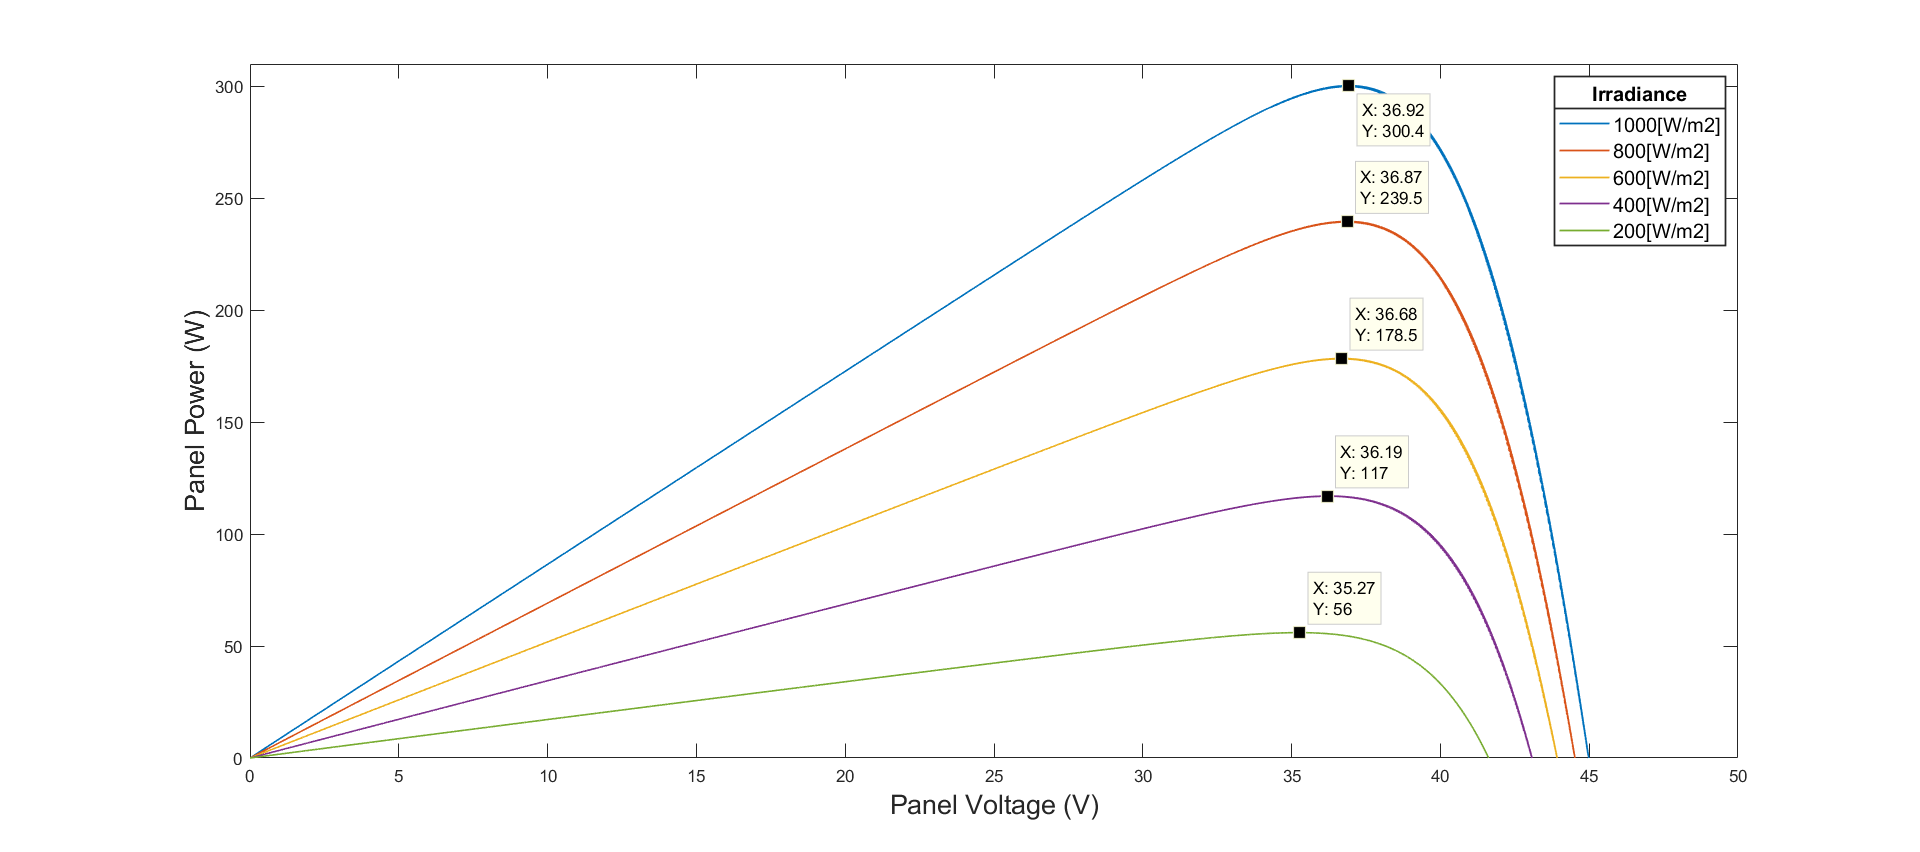
\includegraphics[width=0.8\textwidth]{../Pictures/PV_curves_T25degrees}
		\caption{PV curves for constant T(25deg) and change in I.}
		\label{fig:PVcurves_T25} 
	\end{center}	
\end{figure}

\begin{figure}[H]
	\begin{center}
		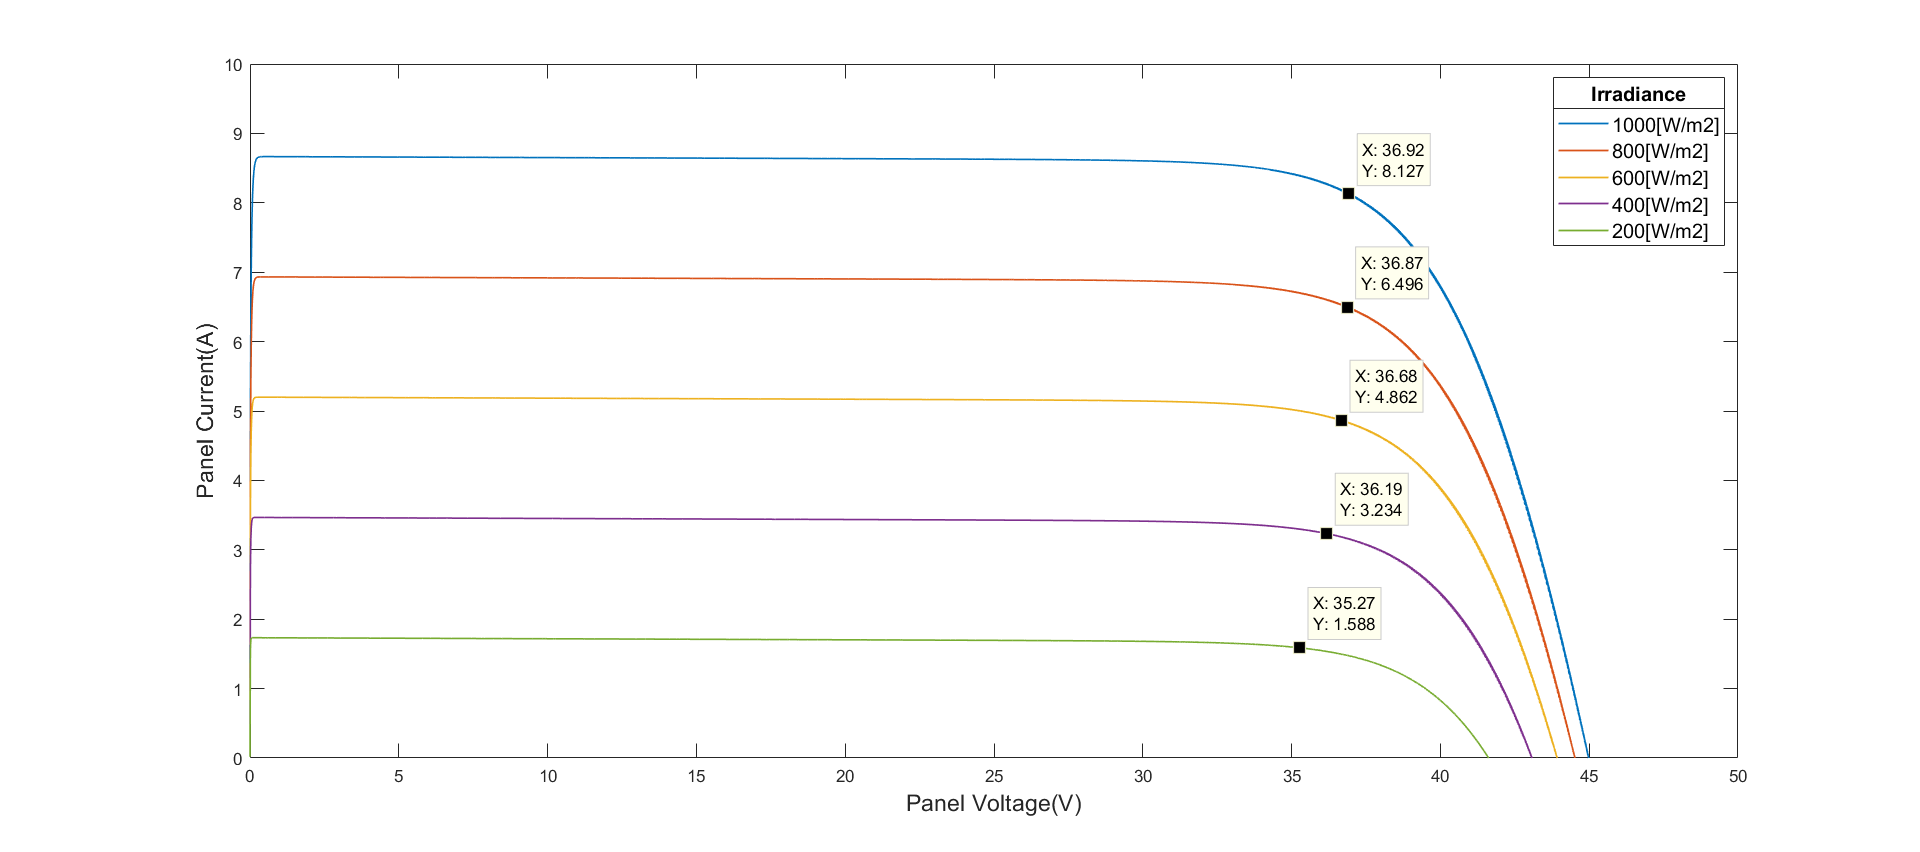
\includegraphics[width=0.8\textwidth]{../Pictures/IV_curves_T25degrees}
		\caption{IV curves for constant T and change in I.}
		\label{fig:IVcurves_T25} 
	\end{center}	
\end{figure}

\begin{figure}[H]
	\begin{center}
		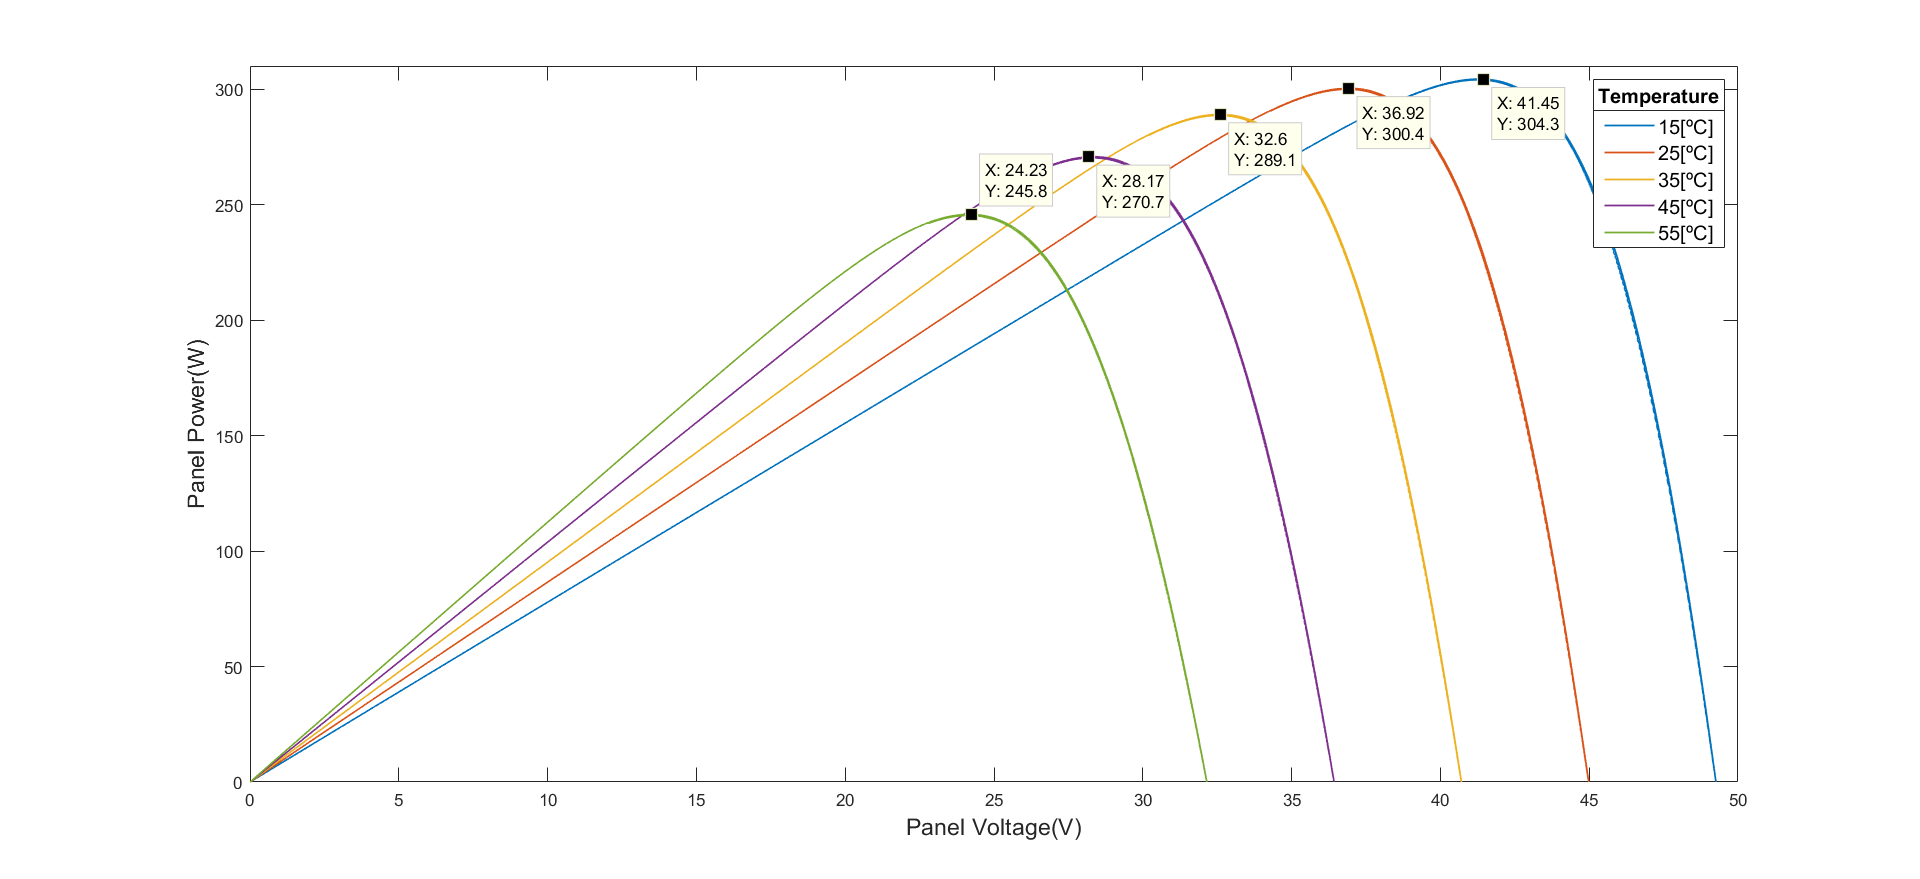
\includegraphics[width=0.8\textwidth]{../Pictures/PV_curves_1000_irradiance}
		\caption{PV curves for constant I(1000) and change in T.}
		\label{fig:PVcurves_Irr1000} 
	\end{center}	
\end{figure}


\begin{figure}[H]
	\begin{center}
		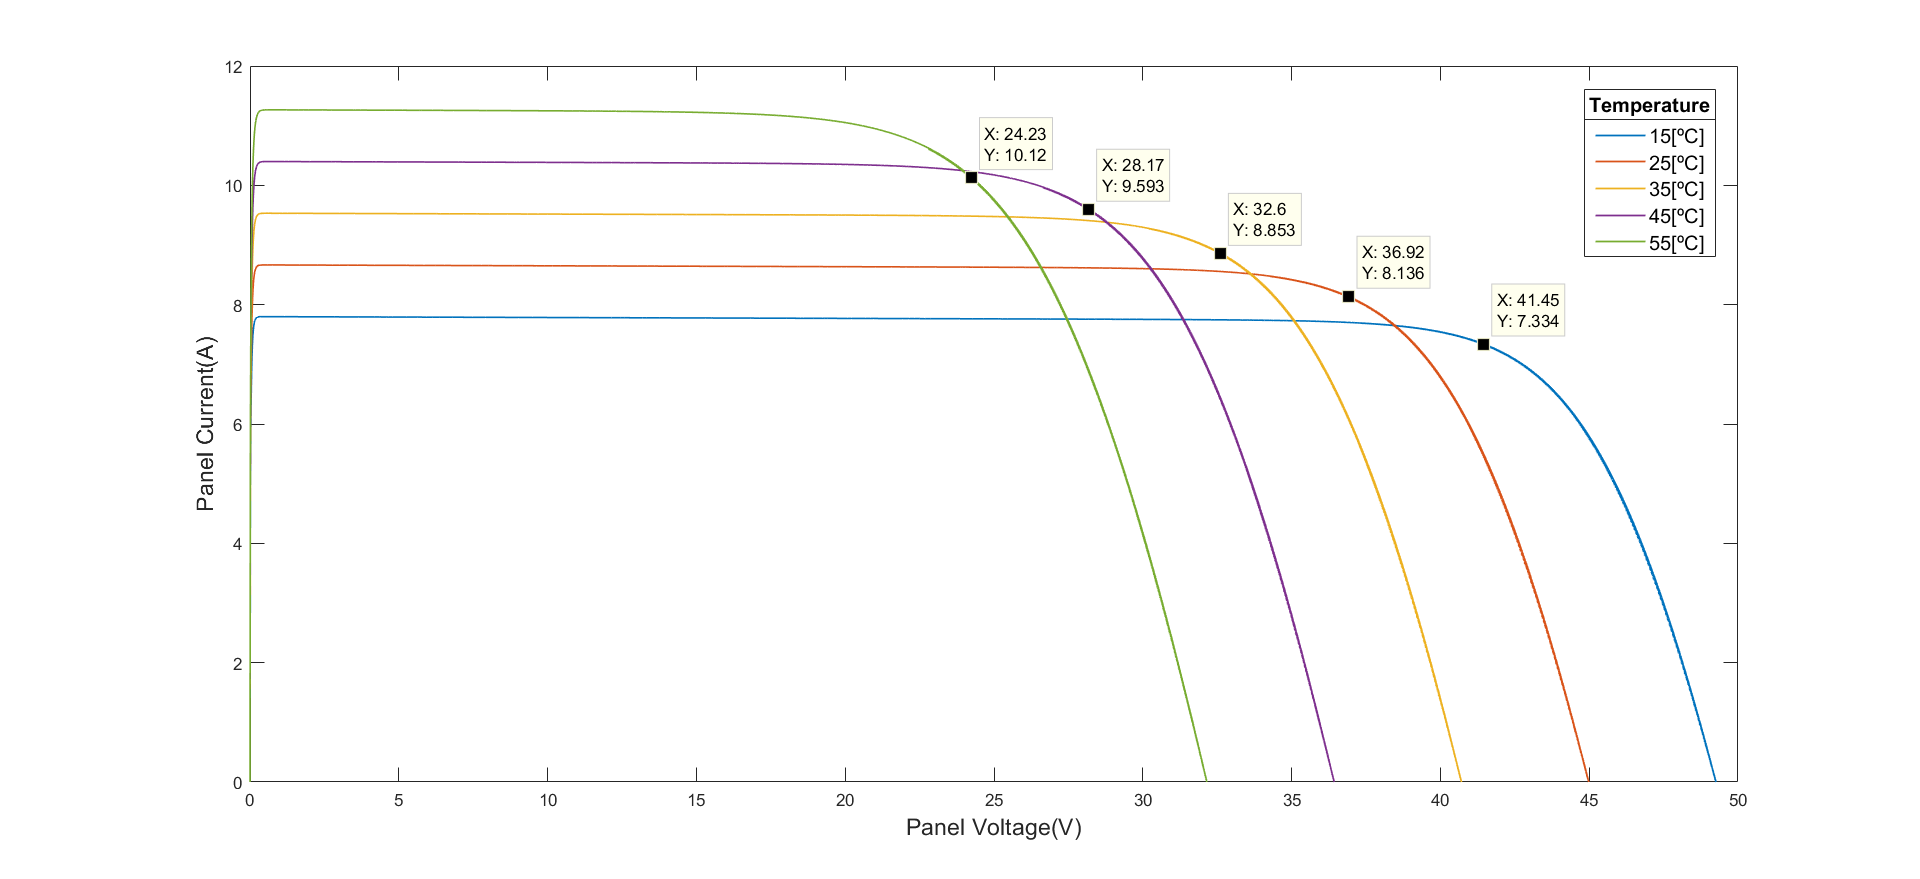
\includegraphics[width=0.8\textwidth]{../Pictures/IV_curves_1000_irradiance}
		\caption{IV curves for constant I(1000) and change in T.}
		\label{fig:IVcurves_Irr1000} 
	\end{center}	
\end{figure}



\subsection{MPPT algorithm results}

THINGS TO WRITE:
\begin{itemize}
	\item For each load value (buck and boost) show the grahs corresponding to change in irradiance, change in temperature 
	\item Graphs: Vin/Iin/Pin. Control variable/Dbuck/Dboost/Vinvsvout
	\item Efficiency of the MPPT in buck and boost
	
\end{itemize}
